\documentclass[]{standalone}

\usepackage{adjustbox}

\usepackage{amsmath}
\usepackage{xfrac}
\usepackage{mathrsfs}

\usepackage{circuitikz}
\usepackage{tikz}
\usetikzlibrary{arrows, patterns, decorations.pathmorphing, backgrounds, positioning, fit, petri, shapes, trees, matrix, chains, decorations, decorations.pathreplacing, decorations.fractals, calc,snakes,trees, decorations.markings}

\usepackage{color}
\definecolor{soton}{RGB}{7,51,71}
\colorlet{comms}{red!50!yellow}
\colorlet{payld}{pink!50!purple}
\colorlet{obdh}{green!50!black}

\begin{document}

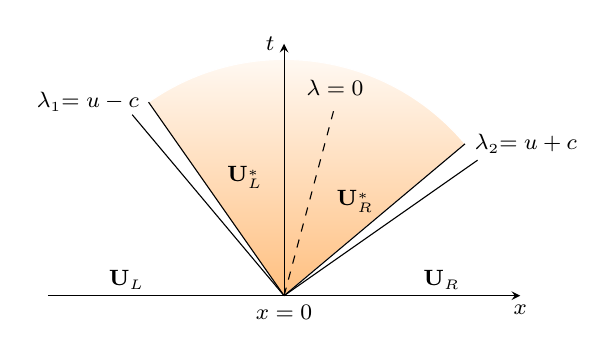
\begin{tikzpicture}

\draw[shade, top color=white, bottom color=yellow!50!red!50, draw=white] (0,0) -+ (40:3) arc (40:90+35:3);

\draw[-stealth] (-3,0) -- (3,0) node[below] {\footnotesize{$x$}};
\draw[-stealth] (0,0) node[below] {\footnotesize{$x=0$}} -- (0,3.2) node[left] {\footnotesize{$t$}};

\draw (0,0) -+ (35:3);
\draw (0,0) -+ (40:3) node[right] {\footnotesize{$\lambda$}\tiny{$_2$}\footnotesize{$=u+c$}};

\draw[dashed] (0,0) -+ (75:2.5) node[above] {\footnotesize{$\lambda=0$}};

\draw (0,0) -+ (90+40:3);
\draw (0,0) -+ (90+35:3) node[left] {\footnotesize{$\lambda$}\tiny{$_1$}\footnotesize{$=u-c$}};

\node at (-0.5, 1.5) {\footnotesize{$\mathbf{U}$}\tiny{$_L^*$}};
\node at (0.9, 1.2) {\footnotesize{$\mathbf{U}$}\tiny{$_R^*$}};
\node at (-2, .2) {\footnotesize{$\mathbf{U}$}\tiny{$_L$}};
\node at (2, .2) {\footnotesize{$\mathbf{U}$}\tiny{$_R$}};

\end{tikzpicture}


\end{document}